\documentclass{article}
\usepackage{amsmath}
\usepackage{graphicx}
\usepackage{config_fancyverbatim}
\usepackage{config_hyperlinks}
\usepackage[final]{pdfpages}

\setlength{\parskip}{\medskipamount}

\title{Mini Project in Database Systems}
\author{Elad Harizy and Abraham Murciano}

\begin{document}

\maketitle

\tableofcontents

\section*{Introduction}

In this document we outline the process we underwent in order to design and create a database. Most of the referenced files can be found on \url{https://github.com/abrahammurciano/ask-us}. File paths will be relative to the repository root directory.

\section{First Stage}

\section{Proposal}

Ask Us is a hypothetical organisation who want to create a website where people can ask and answer questions to the general public on any topic. Our task is to analyse the data needs of such a website, to the ends of creating a database for them along with a website to interface with it.

Ask Us will need to store information on its users, as well as all the questions and answers. They would also like each question and answer to have its own comment thread, for people to contribute helpful information regarding answers as well as for short follow up questions.

All questions, answers, and comments should be scored by the users in some way, so that people can see what posts were considered good by the general public and which were disliked. This should help people evaluate the answers and comments they receive.

Additionally, they would like questions to be organised by topic, where each question can be associated with multiple topics. Users should also be able to follow topics they are interested in, so they can see questions related to their interests.
\section{Entity Relationship Diagram}
\subsection{Entities}
We will have six entities: user, post, question, answer, comment, and topic.

A user is an individual writing a post on Ask Us. The user entity will have five attributes: ID, username, email, password, and points. A user's points are the sum of all the points of all their posts. ID will be the primary key.

A post is anything a user writes. This can either be a question, answer, or comment. The post entity will only have an ID, which is the primary key. The purpose of this entity is mainly so that comments can have their parent post be of any type. (We can comment on questions, answers, and even other comments.)

Questions, answers, and comments will all have the following attributes, aside from the ones we specify below. They will have a body, which is the main text that makes up that post. They will also have a count of the points that they have been awarded by users. They will also have a timestamp which will be the exact date and time a post was made.

The question entity has one other attribute called title, aside from the attributes listed above. Since it is a weak entity, its primary key is the post's ID.

The answer entity has a boolean attribute called accepted, apart from the attributes it has in common with the other post types. Similarly, since it is a weak entity, its primary key is the post's ID.

A comment is typically a short piece of text that a user writes beneath any kind of post. A comment itself has no other attributes, other than the ones above. Once again, since it is a weak entity, its primary key is its post's ID.

A topic is a way for users to categorize their questions, thus getting better targeted responses. A user can also follow a topic of interest. The topic entity will have three attributes: ID, username, and description. ID will once again be the primary key.

\subsection{Relations}
A user can `follow' a topic. In this relation, there can be many topics a user can follow, but it is not mandatory for a user to follow any topic. In the same light, topics can be followed by any number of users.

A user is related to the posts that they write. In this relation, the user can write anywhere from many to no posts. However, a post must be written by exactly one user.

A user is also related to a post by voting on it. The vote relation is a many to many relation, in that a user can vote on many to no posts and a post can be voted on by many to no users.

The comment entity has two relations with the post entity. One relation is called belongs to. This relation represents the fact that a specific comment has a parent post (which may also be a comment). A post can optionally have many comments, but a comment must be a child of exactly one post.

The other relation is an inheritance relation. It is an identifying relation, and is labelled `is a' in figure \ref{erd2}. In this relation, a particular comment is related to exactly one post, meaning that this comment entity `extends' that post, because they are in fact the same post. In this relation, a post does not necessarily have to be related to a comment, since not all posts are comments, but if it is, it must be related to exactly one comment.

Since questions and answers are also types of post, they also have an inheritance relation between themselves and post. This relation is identical to the inheritance relation between comment and post.

Answers must also be related to the questions which they answer. A question can have zero to any number of answers, yet an answer must be related to exactly one question.

Lastly, questions are related to topics. A question must have at least one topic, and a topic can have zero or more questions related to it.

\subsection{Diagram}

There are a few possible ways we can design an entity relationship diagram to suit our needs. One option is what is shown in figure \ref{erd1}. The main aspect to note is that the \textsc{Post} entity has the attributes `body', `timestamp', and `points', which all the three post types don't need to have, since they `inherit' those attributes from \textsc{Post}.

\begin{figure}[p]
	\centering
	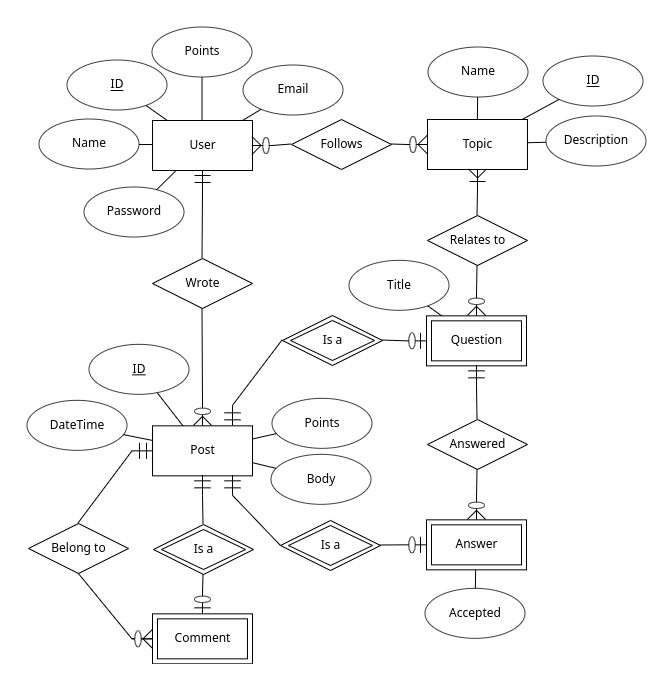
\includegraphics[width=\linewidth]{images/erd1.png}
	\caption{The first design of the ERD}
	\label{erd1}
\end{figure}

However, this may cause inefficiency when retrieving data for any type of post from the database. This is because the attributes of each post would be divided into two tables, requiring us to join the tables to obtain all the data on any particular post.

We therefore tweak the design so that each post type contains all of their fields in the same table, even those that all the post types have in common. This solves the inefficiency because there is no longer a need to join the tables, and this solution still maintains the tables normalized to the same extent that they were prior.

Another consideration we must make is that since a comment is a type of post, and a comment can have child comments, we encounter a cycle in the ERD. Specifically, this means that the depth of a comment thread would have no limit. This can cause issues if we try to query all the descendant comments of any post, since we would need a recursive query for this.

We may consider applying certain techniques such as materialized paths or using a closure table, which would make this kind of query trivial. However, if we give our system some consideration, we can be fairly certain that such queries need not be made.

For example, when the website needs to load all the child comments of any particular question, we are only interested in the top-level comments at first. Retrieving those is also a simple query, since each comment knows its direct parent. Once we have those, the application level can recursively query all the top-level comments of each of those comments, meaning it would obtain all the second-level comments of the question. Similarly, our application can obtain all the comments, regardless of how many levels deep it can be found.

This approach is preferable in our scenario, since obtaining all the descendant comments in one bulk, as techniques like materialized path and closure tables would allow is unhelpful to us. This is because we need to display them in a hierarchical structure, and retrieving them in bulk would then require further processing by the application in order to structure them accordingly.

Another possible modification which we may consider to make the retrieval of comments more efficient is to only allow a single level of comments, or in other words, not allowing for comments to have child comments. However, this would cause a detriment in user experience, as they would be limited to conducting much discussion on some questions or answers.

Therefore we can conclude that the optimal approach would be to maintain the design as we have described above.

Figure \ref{erd2} shows the final design of the entity relationship diagram for the database we are to make for Ask Us. Although the ERD is more complex, it provides the facility to use simpler and more efficient queries to retrieve the data that our system is interested in.

\begin{figure}[p]
	\centering
	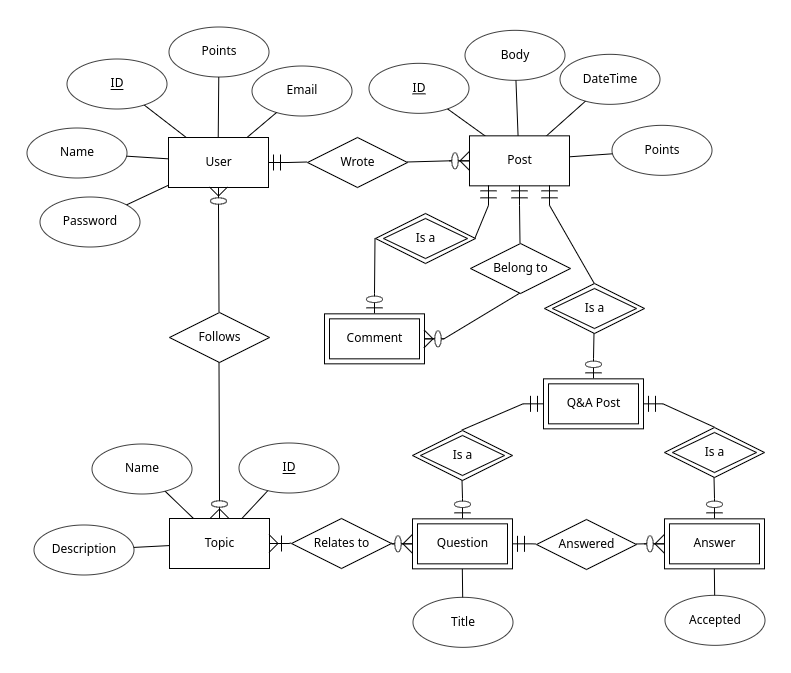
\includegraphics[width=\linewidth]{../../ERD/erd.png}
	\caption{The final ERD for the database for Ask Us}
	\label{erd2}
\end{figure}
\section{Logical Schema}

We are to convert the ERD in the previous section into a logical schema. First we will convert the entities into tables, and then we will add tables for some of the relations where required.
\section{Normalization}
\subsection{Functional Dependencies}
These are the functional dependencies for the \textsc{User} table.
\begin{gather*}
	\text{ID} \to \text{(Name, Email, Password, Points)} \\
	\text{Email} \to \text{(ID, Name, Password, Points)}
\end{gather*}
These are the functional dependencies for the \textsc{Topic} table.
\[\text{ID} \to \text{(Name, Description)}\]
These are the functional dependencies for the \textsc{Comment} table.
\[\text{Post ID} \to \text{(Parent Post ID, Body, Points, TimeStamp)}\]
These are the functional dependencies for the \textsc{Question} table.
\[\text{Post ID} \to \text{(Title, Body, Points, TimeStamp)}\]
These are the functional dependencies for the \textsc{Answer} table.
\[\text{Post ID} \to \text{(Accepted, Question ID, Body, Points, TimeStamp)}\]
The tables for \textsc{Post}, \textsc{Follows}, \textsc{Relates to} and \textsc{Vote} have no non trivial functional dependencies.


\subsection{Third Normal Form}
All the tables above are in 3NF because all the functional dependencies of the form \(X \to Y\) satisfiy the condition ``\(X\) is a superkey''.

The tables for \textsc{Post}, \textsc{Follows}, \textsc{Relates to} and \textsc{Vote} to are also in 3NF since they have no non-trivial functional dependencies.

For the same reason, the tables are all in BCNF.
\section{Physical Schema}

Here we can see the SQL statements which can be used to create the tables we defined above. These statements are specific to Oracle Database.

\subsection{Users Table}

Displayed here is the SQL statement that creates the \verb`users` table. An 8 digit number for the ID (and all ID fields of subsequent tables) is large enough since we will not have more than one million records in the entire database. The ID field is to be generated by the database.

Usernames we limit to twenty characters, and email addresses to 320. This is because 320 characters is the length of the longest possible email address. The \verb`password` field will actually store a base 64 encoded SHA256 hash of the password, which takes 44 bytes.

A reasonable cap for the total number of points a user can accumulate is a ten digit number. This conclusion is based off researching the highest number of points any user has ever accumulated on popular websites which implement similar scoring systems such as Stack Overflow and Reddit, then adding a couple of digits to be on the safe side. By default, a user starts with no points.

\VerbatimInput[label=\fbox{\color{Black}create\_users.sql}]{../../sql/create-table/users.sql}

\subsection{Posts Table}

Below is the SQL statement which creates our table that contains the IDs of all the posts.

\VerbatimInput[label=\fbox{\color{Black}create\_posts.sql}]{../../sql/create-table/posts.sql}

\subsection{Questions Table}

This is the SQL command that generates the questions table. The field \verb`body` is of the CLOB data type, which is short for `character large object'. The \verb`varchar` data type has much smaller length restrictions which would not suffice to allow for long questions.

In this table, we have introduced for the first time the \verb`timestamp` field in SQL. Its data type is \verb`date`, which gives us a date and time representation, accurate up to one second, which is enough for us to record the creation dates of questions (as well as answers and comments). By default, it is assigned the current date and time at the time of insertion of each row.

\VerbatimInput[label=\fbox{\color{Black}create\_questions.sql}]{../../sql/create-table/questions.sql}

\subsection{Answers Table}

Now we come to the SQL statement for the \verb`answers` table. It is mostly identical to the \verb`questions` table, with the exception of the field \verb`accepted` which is a boolean. Since Oracle does not have a built in boolean data type, we use the number data type and limit it to one digit, and we decide that 0 means false and anything else means true.

\VerbatimInput[label=\fbox{\color{Black}create\_answers.sql}]{../../sql/create-table/answers.sql}
\subsection{Report}

Below we can see the report which was generated by PL/SQL Developer after creating all the tables with the SQL statements mentioned in the previous section.

\newlength{\classpagewidth}
\setlength{\classpagewidth}{\pdfpagewidth}
\eject
\pdfpagewidth=115cm
\thispagestyle{empty}
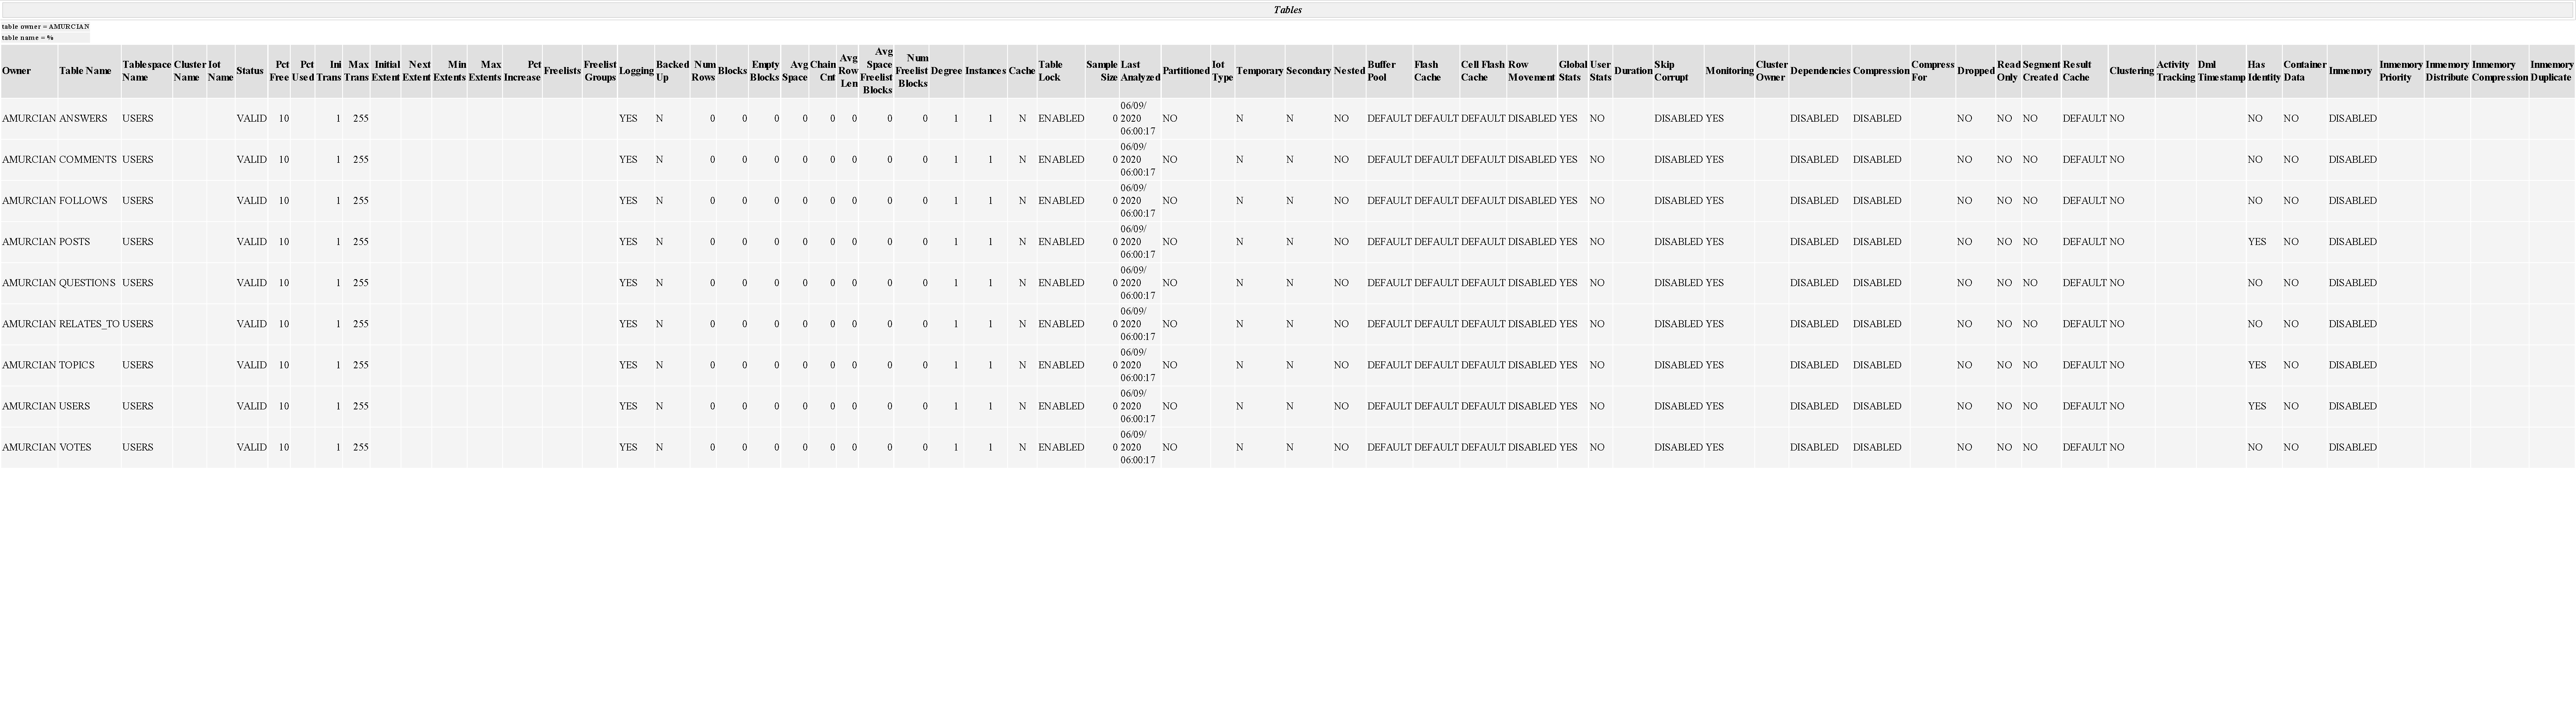
\includegraphics[page=1]{images/report.pdf}

\eject
\pdfpagewidth=\classpagewidth
\section{Populating Tables With Data}

Now that we have successfully created all the necessary data, it is time to fill them with data. We will use a variety of different methods to import data to our tables.

\subsection{Populating Users}

We retrieved a large excel file containing over one hundred thousand users' data from the internet, but since we had no remaining space in the database we had to shrink that file to only one thousand records. Using the PL/SQL Developer tool called ODBC importer we imported the data which we needed into the users table. Not all of the columns provided were necessary to us, so figure \ref{users-odbc} shows which columns we used. The excel file which we used can be found in \verb`/data/users/user_list.xlsx`.

\begin{figure}[hbtp]
	\centering
	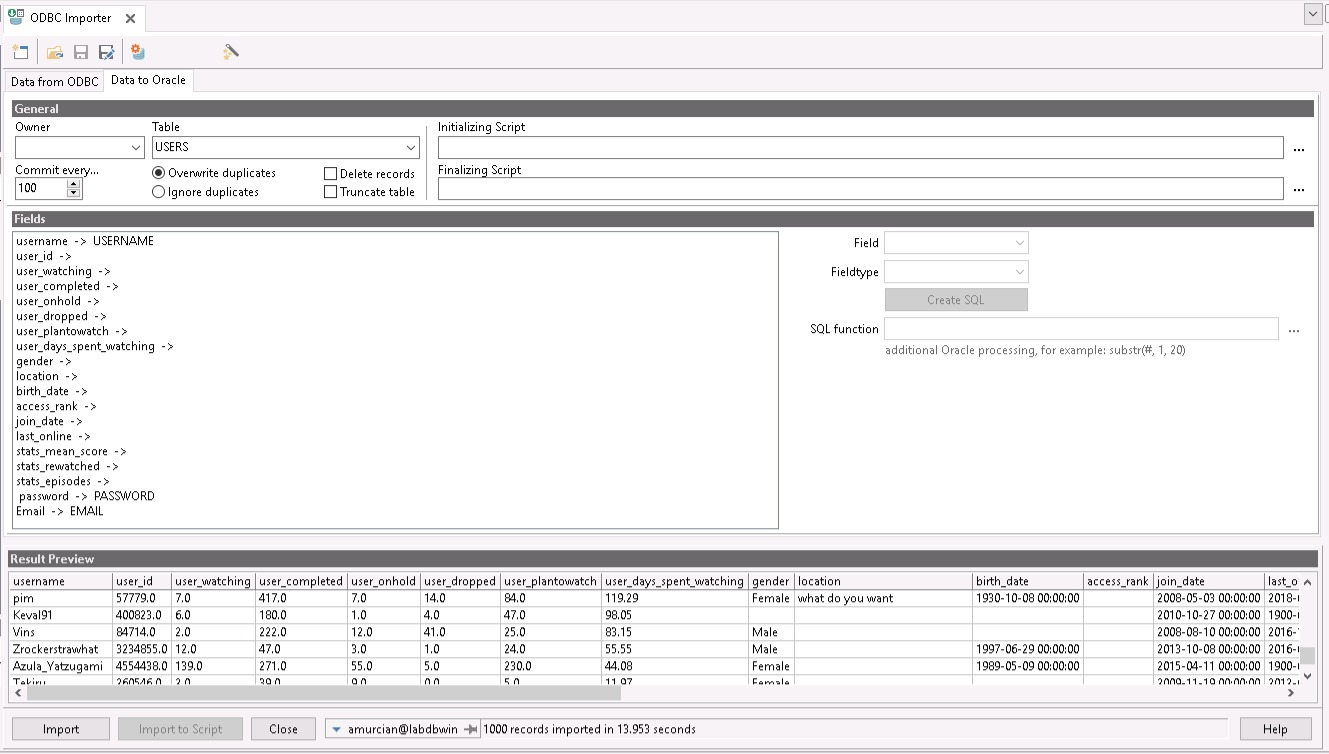
\includegraphics[width=\linewidth]{images/users_odbc.jpeg}
	\caption{A screenshot showing how the ODBC importer imported our data}
	\label{users-odbc}
\end{figure}

\subsection{Populating Posts}

Since this table only contains one column, and that column's value was always generated by the database, this simple script was enough to insert the required number of post IDs into the post table. We originally had inserted over 200,000 but due to severe space constraints we reduced this to 3,000.

\VerbatimInput[label=\fbox{\color{Black}/sql/insert/posts.sql}]{../../sql/insert/posts.sql}

\subsection{Populating Questions}

We were able to obtain a CSV file containing all of the questions which were asked on \LaTeX\ Stack Exchange between January 2010 and September 2020. Since we were restricted on space, we manipulated the CSV file using spreadsheet software to keep only the 1,000 shortest questions. After appending an ID from those which we inserted into the \verb`posts` table to each row, and removing all columns which we do not need, we ran the text importer tool in PL/SQL Developer to add all of the data in the CSV file into the \verb`questions` table.

Figure \ref{questions-text-import} shows the configurations for the text importer which was used to import the questions from our CSV file.

\begin{figure}[htbp]
	\centering
	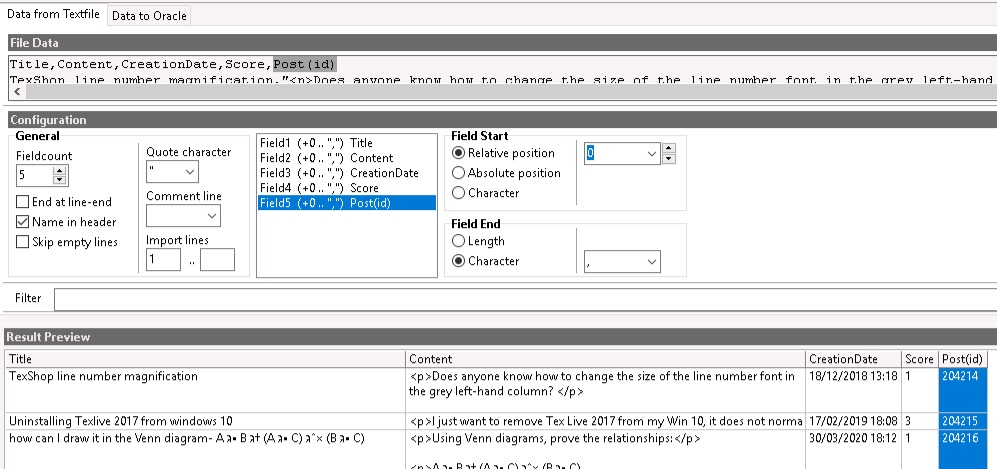
\includegraphics[width=\linewidth]{images/questions_text_import_1.jpeg}
	\vspace{2em}
	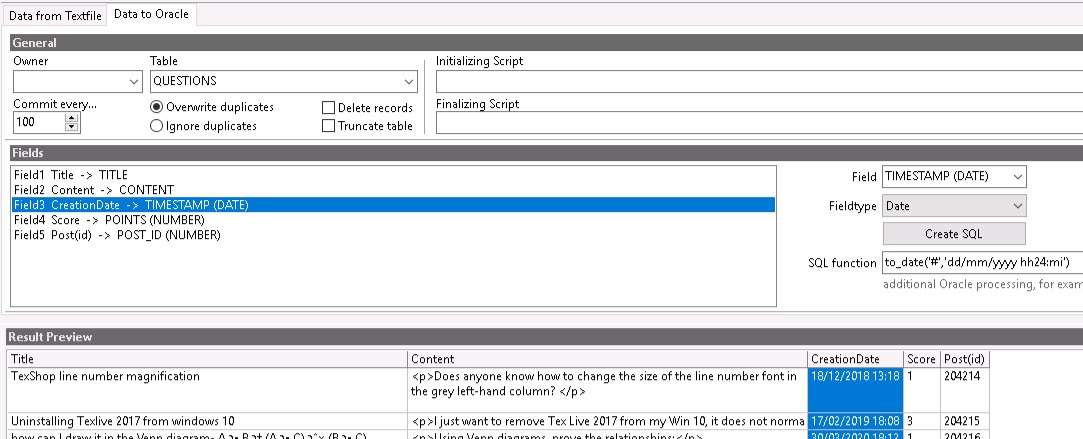
\includegraphics[width=\linewidth]{images/questions_text_import_2.jpeg}
	\caption{The configurations in the text importer for the questions table}
	\label{questions-text-import}
\end{figure}

\subsection{Populating Answers}

We used the data generator tool in PL/SQL developer, as shown in figure \ref{answers-generator}, to populate this table with 1,000 random records.

\begin{figure}[htbp]
	\centering
	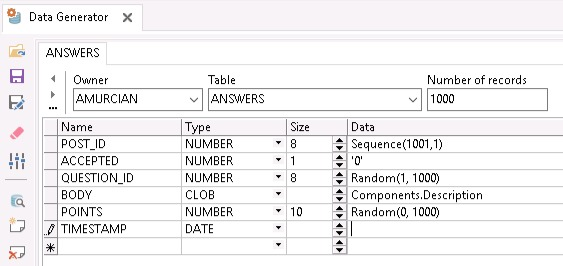
\includegraphics[width=\linewidth]{images/answers_generator.jpeg}
	\caption{The configurations in the data generator tool for the answers table}
	\label{answers-generator}
\end{figure}

\subsection{Populating Comments}

We used the data generator tool to generate 1,000 random comments, but in order to avoid randomly generating circular ancestry with comments, we assigned all comments to a single question. Then we exported the data as a CSV which we then modified so that each comment referenced a post with an ID smaller that the ID of that comment. We then truncated the table to remove the random data, and used the text importer to import the processed CSV in the same way which we imported the questions. This CSV file can be found at \verb`/data/comments/comments.csv`

\subsection{Populating Topics}

We were able to find a large list with 1,547 topics which Quora uses to organise their questions. We obtained it in the form of a plain text file with one line for each topic name. Since it contains duplicates, we can must first remove these. Then we generate some randomised description using the python module called \verb`lorem`. This python code shows exactly how the insert statements were generated. The generated SQL code can be found at \verb`/sql/insert/topics.sql`

\VerbatimInput[label=\fbox{\color{Black}/data/topics/topics\_to\_insert.py}]{../../data/topics/topics_to_insert.py}

\subsection{Populating Votes}

We used the data generator to populate this table. The settings we used to generate the random data is practically identical to those seen in figure \ref{follows-generator}.

\subsection{Populating Follows}

This table was populated using the data generator tool in PL/SQL Developer. We asked the system to generate a number from the users' ID column for the foreign key to that row, and similarly for the other foreign key. Figure \ref{follows-generator} shows the settings we used to generate 1,000 rows.

\begin{figure}[htbp]
	\centering
	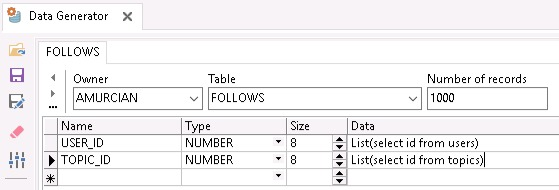
\includegraphics[width=\linewidth]{images/follows_generator.jpeg}
	\caption{Settings used for generating the follows table data}
	\label{follows-generator}
\end{figure}

\subsection{Populating Relates To}

This table also had its data generated in the same way as the \verb`follows` and \verb`relates_to` tables.
\subsection{Validating the Data}

\subsubsection{Negative Points for Certain Questions}

Since the data we used for populating the questions table was obtained from Stack Exchange, some of the questions had a negative number for the points field. However, unlike Stack Overflow, we do not allow negative points, since we only provide users with the ability to up-vote posts, not to down-vote them.

We therefore ran the following SQL statement to negate all the negative values.

\begin{verbatim}
	UPDATE questions SET points = -points WHERE points < 0;
\end{verbatim}

\subsubsection{Circular References in Comment Hierarchy}

Since we randomly generated the comments, and each comment has a field \verb`post_id`, we ended up with some circular references where a comment was its own parent, or a comment's descendant was also an ancestor of that same comment.

In order to solve this, we exported the data as a CSV which we then modified using spreadsheet software and formulae so that each comment referenced a post with an ID smaller its own. We then truncated the table to remove the random data, and used the text importer to import the processed CSV in the same way which we imported the questions. This CSV file can be found at \verb`/data/comments/comments.csv`
\subsection{Backup and Restore}

To test that the data is all in place, we are tasked with creating backups of all the data, then deleting all the data from the database and finally importing it all again.

The exported backup files can be found in the directory \verb`/sql/backup/`, as well as the script which we use to delete all the data, which is called \verb`delete_all.sql`.

\VerbatimInput[label=\fbox{\color{Black}/sql/backup/delete\_all.sql}]{../sql/backup/delete_all.sql}


\section{Second Stage}

\subsection{Queries}

Now that we have built and populated our database, it is time that we use it to retrieve useful information for various users. Therefore we need to create some queries that will perform this task.

\subsubsection{Query Descriptions}

What follows is a description of some queries that will need to be retrieved from the database.

\begin{enumerate}
	\item
	Perhaps the most frequent query that will be used is a search query. In essence, the query would be \emph{obtain all questions whose title or body contain the provided words}.

	\item
	Another query which will be often requested is one that retrieves questions to display on a user's home page. We can describe it as follows. \emph{Retrieve the most popular questions which relate to a topic which a certain user follows}.

	\item
	An alternative query to the previous one with a similar purpose can be to obtain new questions which have not yet been answered instead of popular ones. We can describe this one as follows. \emph{Retrieve the newest unanswered questions which relate to a topic which a certain user follows}.

	\item
	This query is one that will have to be performed every time a question is loaded. \emph{Find all answers which answer the question with a particular ID}.

	\item
	Similar to the previous one, whenever any post is loaded, we would need to query for all the comments on that post. \emph{Select all comments whose parent post has a certain ID}.

	\item
	A user may be interested in viewing all the answers that have been given to the questions they ask, in an `inbox' fashion. \emph{Obtain all answers to questions which were asked by a certain user, sorted from newest to oldest}.

	\item
	Ask Us is interested in sending out a weekly newsletter containing the most popular questions with one of their answers each from the previous week. A query which would obtain these questions would look like this. \emph{Obtain a certain number questions, as well as each of their highest voted answers, which were posted between two weeks ago and one week ago, and received the most votes within a week of their posting}.

	\item
	Ask Us is interested in suggesting trending topics for users to explore. So we would need to write a query that retrieves the following data. \emph{Select the five topics which have had the most posts and votes within the past few days}.

	\subsubsection{Writing the Queries in SQL}

	Next we must convert these queries into SQL code. Wherever user input would have been appropriate, we used a literal instead. The first query searches for a certain search phrase which is provided by the user. Here it is in SQL.

	\VerbatimInput[label=\fbox{\color{Black}/sql/queries/search.sql}]{../sql/queries/search.sql}

	The next queries retrieve information to display on a user's home page, sorted to show the most popular or the newest answers. They are displayed below in SQL.

	\VerbatimInput[label=\fbox{\color{Black}/sql/queries/home\_page\_popularity.sql}]{../sql/queries/home_page_popularity.sql}
	\VerbatimInput[label=\fbox{\color{Black}/sql/queries/home\_page\_new.sql}]{../sql/queries/home_page_new.sql}

	Next we have the query that retrieves all the answers to a question.

	\VerbatimInput[label=\fbox{\color{Black}/sql/queries/answers.sql}]{../sql/queries/answers.sql}

	After that, we created the query that obtains the direct child comments of a particular post.

	\VerbatimInput[label=\fbox{\color{Black}/sql/queries/comments.sql}]{../sql/queries/comments.sql}




\end{enumerate}
\subsection{Indexed Structures}

\subsubsection{Creating Indices}

Our task is to create three indices on our tables in order to improve the time efficiency of the queries we wrote in the previous section. We have decided to create an index on the \verb`points`, \verb`timestamp`, and \verb`author_id` columns of each of the posts' tables. This is because these columns are often the ones ordered by or the ones found in where clauses of the queries above.

Below are the SQL commands which we used to create the indices on all these columns.

\VerbatimInput[label=\fbox{\color{Black}/sql/indices/indices.sql}]{../sql/indices/indices.sql}

\subsubsection{Evaluating Index Efficiency}

Now that we have indices, we are to check if they actually improve efficiency. Table \ref{index-comparison} compares the average run time of five executions of each of the queries before and after the indices were added.

\begin{table}[htbp]
	\centering
	\begin{tabular}{||c||c|c||}
		\hline
		Query & Pre-Index & Post-Index \\
		\hline
		search & 0.0702s & 0.0616s \\
		home\_page\_popularity & 0.0240s & 0.0198s \\
		home\_page\_new & 0.0136s & 0.0130s \\
		answers & 0.0234s & 0.0235s \\
		comments & 0.0232s & 0.0214s \\
		inbox & 0.0864s & 0.0810s \\
		newsletter & 0.0648s & 0.0642s \\
		profile & 0.0220s & 0.0214s \\
		\hline
	\end{tabular}
	\caption{Comparison of execution times before and after indices were created}
	\label{index-comparison}
\end{table}

As the table shows, adding the indices did in fact improve the efficiency of the queries, although the difference is not always significant.
\subsection{Updating the Data}

We now have to write some SQL commands that will manipulate the data we have stored.

\subsubsection{Updating Two Records}

We have written an SQL query that will update the email addresses of users `watchfuleye' and `werlwend'. This command is shown below.

\VerbatimInput[label=\fbox{\color{Black}/sql/update/emails.sql}]{../sql/update/emails.sql}

\subsubsection{Deleting Two Records}

Here is an SQL command that will delete two records from the follows table. This represents the fact that some user does not want to follow some topic any more.

\VerbatimInput[label=\fbox{\color{Black}/sql/update/unfollow.sql}]{../sql/update/unfollow.sql}

\subsubsection{Updating Multiple Records With a Condition}

When we populated the users table, we manually calculated the base 64 encoded SHA256 hash of the string `password' and stored that as all the users' passwords. Now, we will use an SQL command to update the passwords of half of the users (those with an odd ID number) to the first part of their email (before the `@' symbol). Here we present said SQL command.

\VerbatimInput[label=\fbox{\color{Black}/sql/update/passwords.sql}]{../sql/update/passwords.sql}

\subsection{Rollbacks}

We are to write an SQL script which selects a subset of the data from one of our tables, then updates and displays the updated records. Then the script should perform a rollback and display the results of the query again.

We have written a script, which is shown below, which selects all the users who have a username starting with the letter A. Thirty records were found which satisfy this condition. Then the script changes their email address to end in `@aol.com'.

\VerbatimInput[label=\fbox{\color{Black}/sql/rollback/rollback.sql}]{../sql/rollback/rollback.sql}

The results of the first select statement before the update (statement 1) can be found in \verb`/data/rollback/pre-update.csv` and the results of the last select statement after the rollback (statement 5) can be found in \verb`/data/rollback/` \verb`post-rollback.csv`. As expected, they are identical. The reason for this is that when we run the update statement, it is in some temporary state until the changes are committed. Since they are then rolled back, they are never committed, so by the end of the script the data has not changed at all.

Next, we are to run the same script, but instead of the rollback command, we are to commit the changes. This time, the statement five did show the email addresses all ending in `@aol.com'. These results can be seen in the file \verb`/data/rollback/post-commit.csv`. (The results of statement one were identical to the results of statement one from the rollback script.) The reason that this time we do in fact see the updated records with the last query is because we committed the changes, so they have been permanently applied to the table.

Now we are told to grant access to the user \verb`oracle00` and run the rollback script and the commit script as that user.

\begin{verbatim}
	grant select on users to oracle00;
\end{verbatim}

When we ran both scripts, statement two failed in both scripts since that user does not have permission to update records. We were shown an error message saying ``insufficient privileges''.
\subsection{Constraints}

\subsubsection{Adding Constraints}

We are tasked with creating and applying any constraints we deem appropriate to our database. We have already applied all appropriate unique constraints when creating the table, now we will go over all our tables and add check constraints where necessary.

For the users table, we must check that the email address provided is well formed. Meaning that it contains some text, followed by an @ symbol, followed by a domain. We also must ensure that the points are always positive. Here is the alter table command for the users table.

\VerbatimInput[label=\fbox{\color{Black}/sql/constraints/users.sql}]{../sql/constraints/users.sql}

When looking at the questions, answers, and comments table, the only field which needed to be checked was once again the points field. Below are the alter table commands for all three.

\VerbatimInput[label=\fbox{\color{Black}/sql/constraints/questions.sql}]{../sql/constraints/questions.sql}
\VerbatimInput[label=\fbox{\color{Black}/sql/constraints/answers.sql}]{../sql/constraints/answers.sql}
\VerbatimInput[label=\fbox{\color{Black}/sql/constraints/comments.sql}]{../sql/constraints/comments.sql}

\subsubsection{Testing the Constraints}

To test that all our constraints are working correctly, we ran the following commands which would, if successful, violate some of our constraints. First we tried to add a user with an invalid email address.

\VerbatimInput[label=\fbox{\color{Black}/sql/constraints/tests/users.email.sql}]{../sql/constraints/tests/users.email.sql}

This command was unsuccessful and gave the following error message. The reason for this is because the email address provided does not have a valid domain, since there is no dot (.) character.

\begin{verbatim}
	ORA-02290: check constraint (AMURCIAN.CHECK_USERS_EMAIL) violated
\end{verbatim}

Subsequently, we ran an update query to ensure that the points field was not able to become negative.

\VerbatimInput[label=\fbox{\color{Black}/sql/constraints/tests/questions.points.sql}]{../sql/constraints/tests/questions.points.sql}

Similarly, we obtained an error message as follows, since we do not allow negative values in the points field.

\begin{verbatim}
	ORA-02290: check constraint (AMURCIAN.CHECK_QUESTIONS_POINTS)
	violated
\end{verbatim}

We also checked that unique constraints could not be violated by attempting to update a user's username to an already existing one.

\VerbatimInput[label=\fbox{\color{Black}/sql/constraints/tests/users.username.sql}]{../sql/constraints/tests/users.username.sql}

This time, we received a slightly different error message. The reason for the error was because there was already an existing user with the username `werlwend'.

\begin{verbatim}
	ORA-00001: unique constraint (AMURCIAN.SYS_C00574442) violated
\end{verbatim}

Finally, we tested a foreign key constraint by deleting a post from the post table, which had both a child comment and its question record referencing it.

\VerbatimInput[label=\fbox{\color{Black}/sql/constraints/tests/posts.id.sql}]{../sql/constraints/tests/posts.id.sql}

Once again, as expected, we got an error message, because if the record would have been deleted, there would be a question whose post id would not be in the post table, and there would be a comment whose parent post would not exist.

\begin{verbatim}
	ORA-02292: integrity constraint (AMURCIAN.SYS_C00574679) violated
	 - child record found
\end{verbatim}


\end{document}